% =====================================================================
%  Four ideas from statistical physics, tested on stock prices
%  Compile with pdfLaTeX + BibTeX (works as-is on Overleaf).
% =====================================================================
\documentclass[11pt,a4paper]{article}

\usepackage[T1]{fontenc}
\usepackage[utf8]{inputenc}
\usepackage[english]{babel}
\usepackage{mathpazo}
\linespread{1.08}
\usepackage{microtype}
\usepackage[a4paper,top=2.7cm,bottom=2.7cm,left=2.9cm,right=2.9cm]{geometry}
\usepackage{amsmath,amssymb}
\usepackage{graphicx}
\graphicspath{{figures/}}
\usepackage{booktabs,array}
\usepackage{xcolor}
\usepackage[font=small,labelfont=bf,labelsep=period]{caption}
\usepackage{enumitem}
\setlist{itemsep=2pt,topsep=4pt}
\usepackage[numbers,sort&compress]{natbib}
\usepackage[hidelinks]{hyperref}
\usepackage[capitalise,noabbrev]{cleveref}
\usepackage{titlesec}
\titleformat{\section}{\Large\bfseries}{\thesection.}{0.6em}{}
\titleformat{\subsection}{\large\bfseries}{\thesubsection}{0.6em}{}
\setlength{\parskip}{0.35em}
\setlength{\emergencystretch}{2em}
\setcounter{tocdepth}{1}

\newcommand{\dd}{\mathrm{d}}
\newcommand{\myname}{Jesús García Izquierdo}                              
\newcommand{\repo}{\url{https://github.com/jesus-garcia-izquierdo/statistical-physics-of-markets}} 

\title{\textbf{Four ideas from statistical physics,\\ tested on stock prices}}
\author{\myname\\[0.2em]\small Code and data: \repo}
\date{October 2026}

\begin{document}
\maketitle

\begin{abstract}
\noindent I take four textbook ideas from statistical mechanics and condensed matter (Brownian motion, a
heat bath with a fluctuating temperature, an overdamped particle in a harmonic well, and the Ising model)
and check how far each one goes in describing real stock market data: daily Google prices from 2004 to
2008, and monthly values of the S\&P~500 and Nasdaq indices from 1990 to 2022. The random walk gets the
day-to-day behaviour right but badly underestimates extreme days. Letting the ``temperature''
(volatility) fluctuate accounts for a good part of those extremes, and that temperature turns out to be
predictable out of sample while the direction of the price is not. A mean-reverting spread between
the two indices looks like a spring, but it does not pass a comparison with random walks. The Ising model,
read as a market of investors who copy each other, reproduces bubbles, crashes, a diverging response to
news and hysteresis. Everything here is reproduced by four short Python scripts.
\end{abstract}

\tableofcontents

% =====================================================================
\section{Motivation}
% =====================================================================

I'm a master's student in condensed matter physics, and this project started with a simple question:
how much of the statistical mechanics I've been studying actually survives contact with real market data?
There is a whole field built around that question, usually called econophysics
\cite{mantegna2000,bouchaud2003}, and a lot of it is quite technical. Here I wanted to do the opposite:
pick a few ideas that any physics student already knows, apply them carefully to real prices, and be honest
about where they work and where they don't.

The connection between physics and markets is older than it looks. The first mathematical theory of
Brownian motion was not Einstein's 1905 paper \cite{einstein1905}. It was Louis Bachelier's PhD thesis in
1900, and it was about prices on the Paris stock exchange \cite{bachelier1900}.

\subsection{The minimum amount of finance needed}

I'll keep the finance to a minimum and define things as they come up. A \emph{stock} is a small piece of
ownership of a company. It is traded on an exchange that works like a continuous auction: the price is
just the last value at which a buyer and a seller agreed. When more people want to buy than to sell, the
price goes up, and vice versa. That's really all we need.

Instead of the price $P_t$ itself, I work with the daily \emph{log-return}
\begin{equation}
r_t=\ln\frac{P_t}{P_{t-1}} .
\end{equation}
For small moves this is basically the percentage change (from 100 to 102, $r=0.0198$). The reason for the
log is that returns over consecutive days add up, like the steps of a walker. The \emph{volatility}
$\sigma$ is the standard deviation of $r_t$. For Google in 2004--2008, $\sigma=2.36\%$ per day. A
\emph{stock index} (S\&P~500, Nasdaq) is a weighted average of many stock prices and works as a
thermometer for the market as a whole.

\subsection{Data and layout}

Both datasets ship with \texttt{matplotlib}, so nothing needs to be downloaded:
\begin{itemize}
\item daily closing prices of Google from its IPO (August 2004) to October 2008: 1047 days, 1046 returns.
This covers a period of strong growth and the start of the 2008 financial crisis;
\item monthly values of the S\&P~500 and the Nasdaq from 1990 to 2022 (391 months), which include the
dot-com bubble around 2000.
\end{itemize}
Each of the next four sections follows the same order: the physics, the translation into market language,
and then the data. \Cref{tab:plan} is the map.

\begin{table}[ht]
\centering\small
\caption{The four ideas and the script that goes with each one.}
\label{tab:plan}
\begin{tabular}{@{}l>{\raggedright\arraybackslash}p{3.5cm}>{\raggedright\arraybackslash}p{5.0cm}>{\raggedright\arraybackslash}p{4.0cm}@{}}
\toprule
& Physics & Market & Script \\
\midrule
\S\ref{sec:walk} & Brownian motion, diffusion & prices are unpredictable; risk grows as $\sqrt t$ & \texttt{01\_paseo\_aleatorio.py}\\
\S\ref{sec:temp} & heat bath with varying $T$ & calm and turbulent periods; extreme days & \texttt{02\_temperatura.py}\\
\S\ref{sec:spring} & particle on a spring (Langevin) & price gaps that close over time & \texttt{03\_muelle.py}\\
\S\ref{sec:ising} & Ising model & herding, bubbles and crashes & \texttt{04\_ising.py}\\
\bottomrule
\end{tabular}
\end{table}

% =====================================================================
\section{The price as a Brownian particle}
\label{sec:walk}
% =====================================================================

\subsection{Physics: a walker with no memory}

A pollen grain in water gets kicked by the surrounding molecules. Each kick is random and has nothing to do
with the previous one. After $t$ time steps its position is
\begin{equation}
x_t=x_0+\xi_1+\xi_2+\dots+\xi_t ,
\end{equation}
with independent steps $\xi_k$ of mean $\mu$ and variance $\sigma^2$. Since variances of independent
variables add,
\begin{equation}
\langle(x_t-x_0-\mu t)^2\rangle=\sigma^2\,t ,
\label{eq:diffusion}
\end{equation}
so the mean squared displacement grows linearly in time and the typical displacement grows as $\sqrt t$. In
the continuum limit the probability density obeys the diffusion equation,
\begin{equation}
\frac{\partial p}{\partial t}=D\,\frac{\partial^2p}{\partial x^2},\qquad D=\frac{\sigma^2}{2},
\end{equation}
whose solution starting from a point is a Gaussian of width $\sqrt{2Dt}$. And by the central limit theorem
the sum of many steps is Gaussian even if each individual step is not.

\subsection{Market version}

Take $x_t=\ln P_t$. Then each step is a daily return, $\xi_t=r_t$, and Bachelier's model says returns are
independent.

Why should they be? The argument is simple. Suppose everyone knew that Google would go up 3\%
tomorrow. Everybody would buy today, and that wave of buyers would push the price up \emph{today}. The
predicted move disappears as soon as it is predicted. If all public information is already in today's price,
only new information can move it tomorrow, and new information is unpredictable by definition. This is the
efficient market hypothesis \cite{fama1970}. It doesn't have to be exactly true, but it gives a reason to
expect returns to look like random kicks.

\begin{table}[ht]
\centering\small
\caption{Dictionary for this section.}
\begin{tabular}{@{}ll@{}}
\toprule
Physics & Market \\
\midrule
position $x_t$ & log-price $\ln P_t$\\
step $\xi_t$ & daily return $r_t$\\
molecular kicks & news, buy and sell orders\\
drift $\mu$ & average trend of the price\\
diffusion coefficient $D=\sigma^2/2$ & half the squared volatility\\
\bottomrule
\end{tabular}
\end{table}

A quick test you can try on yourself: in \cref{fig:walks}, three of the curves are random walks with the
same mean and volatility as Google, and one is the real Google price. I couldn't tell them apart without
looking at the code. The answer is in the caption.

\begin{figure}[ht]
\centering
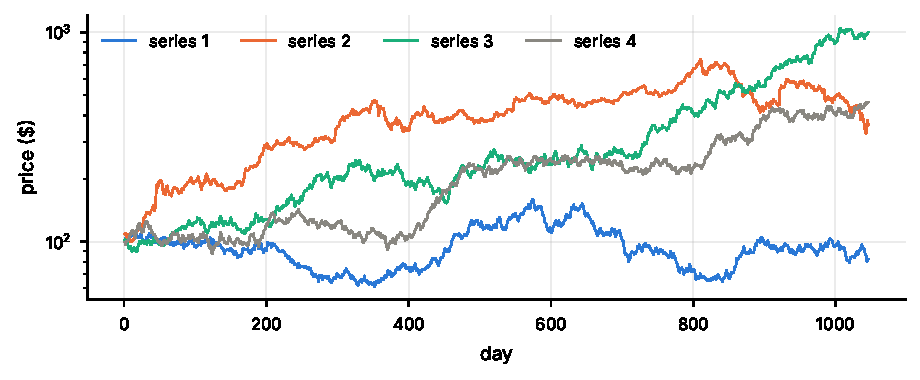
\includegraphics[width=0.95\textwidth]{fig1_paseos.pdf}
\caption{Three simulated random walks with Google's mean and volatility, plus the real Google price
(Aug 2004 to Oct 2008), all starting at \$100. Log scale. The real one is series 2.}
\label{fig:walks}
\end{figure}

\subsection{Risk grows like the square root of time}

\Cref{eq:diffusion} has a direct practical consequence. With a daily volatility $\sigma$, the volatility
over $t$ days is $\sigma\sqrt t$, not $\sigma t$. For Google, that's $2.36\%$ over a day, $10.8\%$ over a
month (21 trading days) and $37.5\%$ over a year (252 trading days). If risk grew linearly, the yearly
number would be $595\%$. This square-root rule is what banks use to convert risk between horizons.

There's a second, less obvious consequence. The drift grows as $\mu t$ but the noise only as
$\sigma\sqrt t$, so their ratio grows as $\sqrt t$. For Google, $\mu=0.12\%$ per day: on a single day the
trend is twenty times smaller than the noise, and invisible. Over a year the accumulated trend ($31\%$) is
comparable to the noise ($37\%$). I think this is the cleanest way to see why long-term investing and
short-term speculation are such different games: on short time scales, it's almost all noise.

\subsection{Checking it against the data}

The model makes two predictions I can test directly with the 1046 Google returns (\cref{fig:diffusion}).

\paragraph{No memory.} The autocorrelation $C(\tau)$ measures how much today's return resembles the one
$\tau$ days later. For a random walk $C(\tau)=0$, and with a finite sample of $n$ points the estimate falls
inside $\pm1.96/\sqrt n=\pm0.061$ about 95\% of the time. I get $C(1)=0.024$. Out of the first 20 lags,
2 fall slightly outside the band, which is what you'd expect by chance.

\paragraph{Diffusion.} I computed the variance of returns summed over $k$ days, for $k=1,\dots,60$. On a
log--log plot, linear growth is a straight line of slope 1. The fitted slope is $1.10$. The small excess is
probably due to the long trends of this particular period, which make multi-day returns add up a bit more
than in a pure walk.

\begin{figure}[ht]
\centering
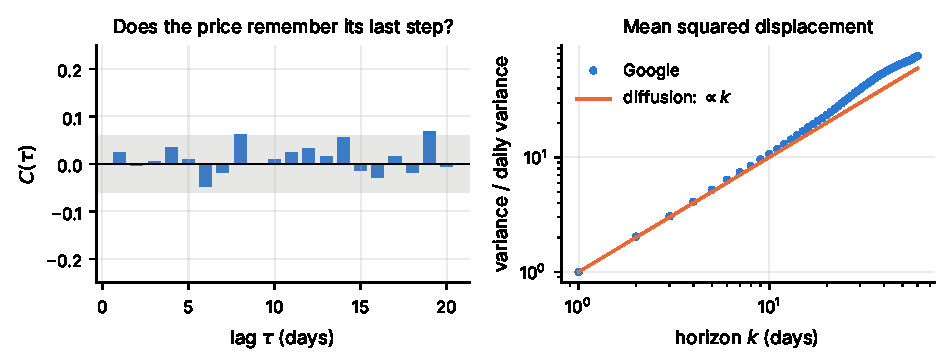
\includegraphics[width=\textwidth]{fig1_difusion.pdf}
\caption{Left: autocorrelation of Google's daily returns; the grey band is what you get with no memory.
Right: variance of $k$-day returns divided by the daily variance, against the diffusion line.}
\label{fig:diffusion}
\end{figure}

\subsection{Where it breaks: extreme days}

The third prediction is Gaussian returns, and this is where the model fails, in the place where it matters
most. Measuring each return in standard deviations, $z=(r-\mu)/\sigma$, and counting large moves:

\begin{table}[ht]
\centering\small
\caption{Google days with a move larger than the threshold (either direction), observed and expected for
Gaussian returns.}
\label{tab:extremes}
\begin{tabular}{@{}lcc@{}}
\toprule
Threshold & Observed & Expected (Gaussian)\\
\midrule
$|z|>3$ & 16 & 2.8\\
$|z|>4$ & 6 & 0.07\\
$|z|>5$ & 4 & 0.0006\\
\bottomrule
\end{tabular}
\end{table}

A move larger than $5\sigma$ should happen about once every 6900 years if returns were Gaussian. It
happened four times in four years. \Cref{fig:tails} shows the same thing on a log scale: the Gaussian is a
parabola that drops fast, the data have \emph{fat tails}. The excess kurtosis (zero for a Gaussian) is
$7.6$. Mandelbrot pointed this out in 1963 for cotton prices \cite{mandelbrot1963}, and it's one of the
most robust facts about financial markets \cite{cont2001}.

\begin{figure}[ht]
\centering
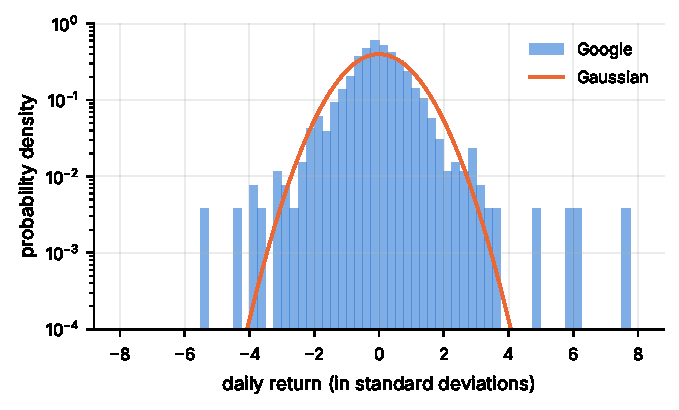
\includegraphics[width=0.7\textwidth]{fig1_colas.pdf}
\caption{Histogram of Google's daily returns in standard deviations versus the Gaussian, log scale. The
isolated bars at both ends are days a Gaussian would essentially never produce.}
\label{fig:tails}
\end{figure}

So which assumption of the central limit theorem is broken? It needs steps that are independent
\emph{and identically distributed}. As the next section shows, the second one is the problem: not all days
are alike, because the ``temperature'' of the market changes.

% =====================================================================
\section{Volatility as temperature}
\label{sec:temp}
% =====================================================================

\subsection{Physics: a particle in a heat bath}

In a gas at temperature $T$, each velocity component of a molecule follows the Maxwell--Boltzmann
distribution, a Gaussian with $\langle v^2\rangle=k_BT/m$. Temperature is literally the width of the
velocity distribution.

Now suppose the temperature of the bath is not fixed but drifts slowly up and down, and we collect
velocities over a long time. What we get is a \emph{mixture} of Gaussians with different widths, and a
mixture of Gaussians is not a Gaussian. It has more weight at the centre (cold periods) and much more in
the tails (hot periods). In statistical physics this is called \emph{superstatistics} \cite{beck2003}.

\subsection{Market version}

The daily return plays the role of the velocity and the volatility plays the role of temperature,
$\sigma^2\leftrightarrow k_BT$. A ``hot'' market is one where prices move a lot every day, in either
direction: during a crisis, around elections, or just before a company publishes its results. A ``cold''
market is a quiet one.

\begin{table}[ht]
\centering\small
\caption{Dictionary for this section.}
\begin{tabular}{@{}ll@{}}
\toprule
Physics & Market \\
\midrule
molecular velocity & daily return\\
temperature, $k_BT/m$ & squared volatility, $\sigma^2$\\
bath heating up and cooling down & calm periods and crises\\
mixture of temperatures & fat tails\\
relaxation time of the temperature & how long a turbulent period lasts\\
\bottomrule
\end{tabular}
\end{table}

\subsection{A thermometer for the market}

The crudest thermometer is the standard deviation of the previous 20 daily returns (about one month).
\Cref{fig:thermometer} shows it for Google, annualized. It is far from constant: it ranges from $12\%$ in
the calm of 2007 to $86\%$ in October 2008. And turbulent days don't come alone, they come in bursts.
This is what people in finance call \emph{volatility clustering}.

\begin{figure}[ht]
\centering
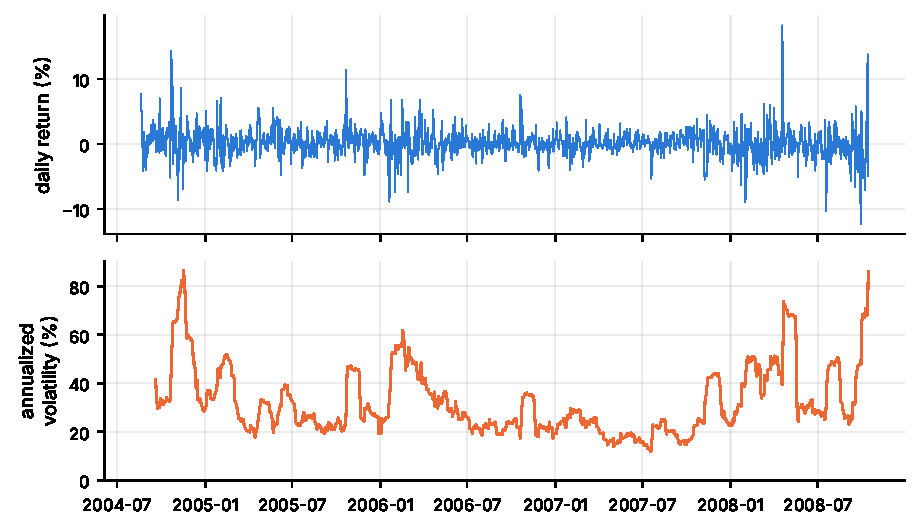
\includegraphics[width=0.95\textwidth]{fig2_termometro.pdf}
\caption{Top: Google's daily returns. Bottom: their ``temperature'', the volatility of the previous 20
days (annualized).}
\label{fig:thermometer}
\end{figure}

\subsection{The sign has no memory, the size does}

We saw that $r_t$ has no memory. Its size $|r_t|$ is a different story (\cref{fig:memory}). The
autocorrelation of $|r_t|$ is $0.148$ at one day and stays positive for weeks, with an average of $0.093$
over the first 20 lags, compared with $0.011$ for $r_t$. A turbulent day tends to be followed by another
turbulent day, even if we can't say which way it will go.

\begin{figure}[ht]
\centering
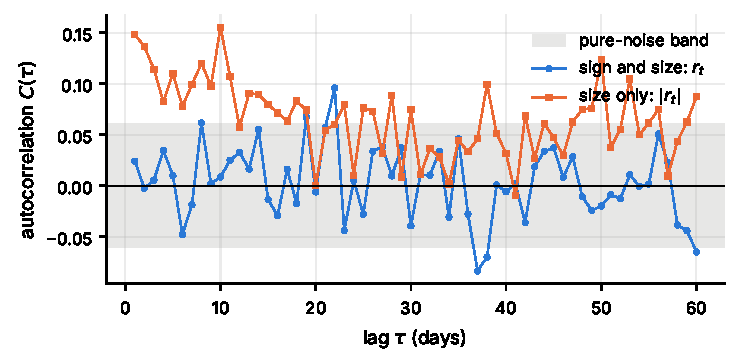
\includegraphics[width=0.75\textwidth]{fig2_memoria.pdf}
\caption{Autocorrelation of the return $r_t$ (blue) and of its size $|r_t|$ (orange) for lags from 1 to
60 days. Grey: the band compatible with pure noise.}
\label{fig:memory}
\end{figure}

In physics language there's a separation of time scales: the ``velocity'' decorrelates in a day, but the
``temperature'' is a slow variable that changes over weeks or months.

\subsection{A toy model: two temperatures are enough}

Take the simplest possible market with two temperatures: $80\%$ of the days are cold, with $\sigma=1.5\%$,
and $20\%$ are hot, with $\sigma=4\%$. Each day on its own is Gaussian. Then:
\begin{itemize}
\item the total variance is the average of the variances, $0.8\times1.5^2+0.2\times4^2=5$, so
$\sigma_{\text{total}}=2.24\%$, close to Google's;
\item the fourth moment of each Gaussian is $3\sigma^4$, so for the mixture it is
$3(0.8\times1.5^4+0.2\times4^4)=165.75$ and the excess kurtosis is $165.75/5^2-3=3.6$;
\item the probability of a daily drop larger than $8\%$ is $0.46\%$ for the mixture and $0.017\%$ for a
single Gaussian with the same total volatility. That's a factor of 26.
\end{itemize}
\Cref{fig:mixture} shows it. In the centre the mixture and the Gaussian look the same, but the tails are
dominated by the hot days. You don't need any special mechanism for extreme days: it's enough for the
temperature to change.

\begin{figure}[ht]
\centering
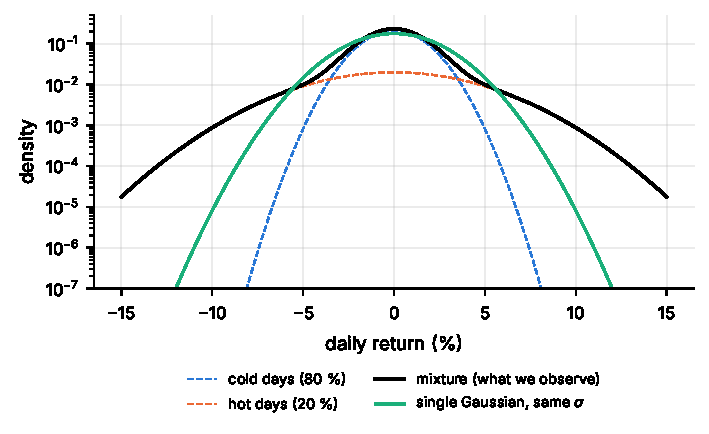
\includegraphics[width=0.72\textwidth]{fig2_mezcla.pdf}
\caption{A mixture of $80\%$ cold days ($\sigma=1.5\%$) and $20\%$ hot days ($\sigma=4\%$), against a single
Gaussian with the same total volatility. Log scale.}
\label{fig:mixture}
\end{figure}

With a continuous distribution of temperatures it gets even better. If the inverse variance
$\beta=1/\sigma^2$ (the analogue of $1/k_BT$) follows a gamma distribution, the mixture is exactly a
Student $t$ distribution,
\begin{equation}
p(r)=\int_0^\infty\sqrt{\frac{\beta}{2\pi}}\,e^{-\beta r^2/2}\,f(\beta)\,\dd\beta
\ \propto\ \left(1+\frac{r^2}{\nu s^2}\right)^{-(\nu+1)/2},
\end{equation}
whose tails decay as a power law $|r|^{-(\nu+1)}$ rather than as $e^{-r^2}$. Fat tails from equilibrium
physics, as long as the temperature is allowed to fluctuate \cite{beck2003}.

\subsection{A thermometer with memory}

The 20-day thermometer treats a day three weeks ago exactly like yesterday. A better one, and the standard
model in finance, is GARCH \cite{engle1982,bollerslev1986}:
\begin{equation}
\sigma_t^2=\omega+\alpha\,r_{t-1}^2+\beta\,\sigma_{t-1}^2 .
\label{eq:garch}
\end{equation}
Today's temperature is a background level ($\omega$), plus yesterday's ``kick'' ($r_{t-1}^2$: a big move
heats the market up), plus yesterday's temperature (inertia). Subtracting the long-run level
$\bar\sigma^2=\omega/(1-\alpha-\beta)$ from both sides, it becomes a relaxation law, like Newton's cooling
with random kicks:
\begin{equation}
\sigma_t^2-\bar\sigma^2=(\alpha+\beta)\left(\sigma_{t-1}^2-\bar\sigma^2\right)+\alpha\left(r_{t-1}^2-\sigma_{t-1}^2\right).
\end{equation}
The first term pulls the temperature back to its mean; the second is a zero-mean kick.

A maximum-likelihood fit to Google gives $\alpha=0.057$ and $\beta=0.935$. The persistence
$\alpha+\beta=0.992$ is very close to 1, so the temperature relaxes slowly: a turbulent spell loses half
of its excess in $\ln(1/2)/\ln(0.992)\approx90$ trading days, about four months.

\subsection{What temperature explains, and what it doesn't}

If a fluctuating temperature were the only source of fat tails, dividing each return by its own day's
temperature, $z_t=r_t/\sigma_t$, should give back a Gaussian. \Cref{fig:normalized} shows that it helps,
but only partly: the excess kurtosis goes from $7.6$ to $6.1$.

\begin{figure}[ht]
\centering
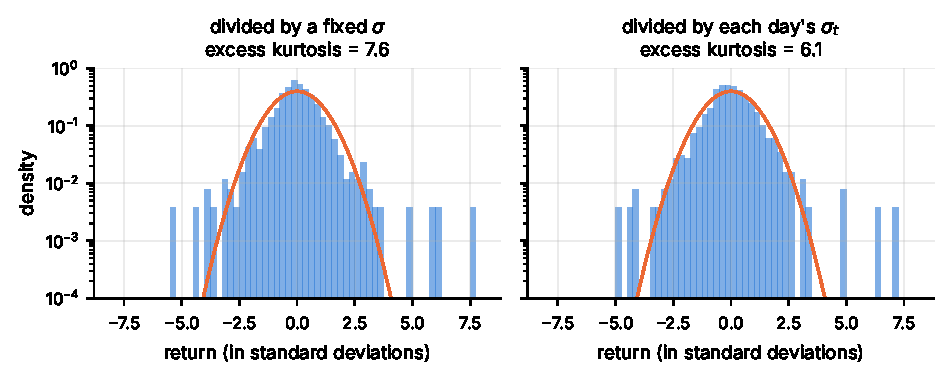
\includegraphics[width=0.95\textwidth]{fig2_normalizar.pdf}
\caption{Google returns divided by a fixed volatility (left) and by each day's GARCH temperature (right),
against the Gaussian.}
\label{fig:normalized}
\end{figure}

The interesting part is to look at \emph{which} days remain extreme:

\begin{table}[ht]
\centering\small
\caption{Google's six most extreme days, in standard deviations.}
\label{tab:six}
\begin{tabular}{@{}lrrl@{}}
\toprule
Date & fixed $\sigma$ & that day's $\sigma_t$ & What happened\\
\midrule
2008-04-18 & $+7.7$ & $+7.2$ & quarterly earnings report\\
2004-10-22 & $+6.0$ & $+4.9$ & quarterly earnings report\\
2008-10-13 & $+5.8$ & $+3.4$ & market-wide rebound after bank bailouts\\
2008-09-29 & $-5.3$ & $-4.4$ & market-wide crash (2008 crisis)\\
2005-10-21 & $+4.8$ & $+6.4$ & quarterly earnings report\\
2008-07-18 & $-4.4$ & $-4.9$ & quarterly earnings report\\
\bottomrule
\end{tabular}
\end{table}

There are two kinds of days here. The two crisis days happened when the market was already very hot, and
once measured against that day's temperature they stop being so extreme ($5.8\to3.4$). That's exactly the
superstatistics picture. The other four are the days right after Google published its quarterly earnings
(how much money it made in the previous three months). That information arrives all at once, on a known
date but with unknown content, and the price jumps. No thermometer based on the past can see that coming.
In physics terms these aren't thermal fluctuations, they're impulsive external forces: a sharp kick on the
particle rather than noise from the bath.

\subsection{Tomorrow's temperature can be predicted}

To test this honestly, I fitted GARCH on the first half of the data only (up to September 2006) and used
it to predict, for each day of the second half, the next day's temperature. Then I split those days into
five equal groups, from coldest to hottest predicted, and compared with what actually happened
(\cref{fig:prediction}).

\begin{figure}[ht]
\centering
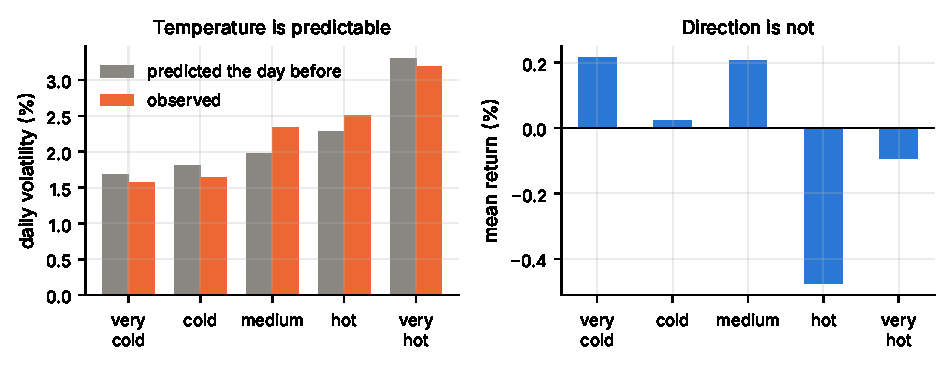
\includegraphics[width=0.95\textwidth]{fig2_prediccion.pdf}
\caption{Second half of the data (Sept 2006 to Oct 2008), never used in the fit. Days are grouped by the
temperature predicted the day before. Left: predicted and observed volatility per group. Right: mean
return per group.}
\label{fig:prediction}
\end{figure}

Predicted temperature goes from $1.68\%$ to $3.31\%$ per day across the groups, and the observed one from
$1.58\%$ to $3.20\%$. The mean return, on the other hand, jumps around with no order ($+0.22\%$,
$+0.02\%$, $+0.21\%$, $-0.48\%$, $-0.09\%$). Knowing tomorrow will be turbulent tells you nothing about
whether it'll go up or down. If I had to keep one result from this whole project it would be this one:
the direction of the price is close to unpredictable, but its temperature is not. In practice you could
use it like a thermostat, investing less when the market heats up and more when it cools down, to keep the
risk roughly constant.

% =====================================================================
\section{Prices that come back: a particle on a spring}
\label{sec:spring}
% =====================================================================

\subsection{Market version first}

A single stock price behaves like a free walker: nothing pulls it back anywhere. But some quantities can't
drift away forever. The typical case is the price difference between two very similar things, like two
oil companies, or the same product sold in two places. If the gap gets too large, someone will buy the
cheap one and sell the expensive one, and in doing so push the two prices together. That's called
\emph{arbitrage}, and it acts as a restoring force. The gap between two related prices is usually called a
\emph{spread}.

\subsection{Physics: Langevin with a spring}

Picture a pollen grain attached to a spring of constant $k$, in a very viscous liquid like honey. Three
forces act on it: the spring $-k(x-\mu)$, friction $-\gamma\dot x$, and thermal kicks $\eta(t)$:
\begin{equation}
m\ddot x=-\gamma\dot x-k(x-\mu)+\eta(t) .
\end{equation}
In a viscous liquid inertia doesn't matter, so the $m\ddot x$ term can be dropped. Dividing by $\gamma$ we
get the Ornstein--Uhlenbeck equation \cite{uhlenbeck1930}:
\begin{equation}
\dd x=-\theta\,(x-\mu)\,\dd t+\sigma\,\dd W,\qquad \theta=\frac{k}{\gamma},\qquad
\sigma^2=\frac{2k_BT}{\gamma}.
\label{eq:ou}
\end{equation}
$\dd W$ is white noise, and the last relation is Einstein's fluctuation--dissipation relation: the same
fluid that slows the particle down is the one shaking it, so noise, friction and temperature are tied
together \cite{uam_me4,gardiner2009}. $\theta$ is how fast the spring brings the particle back, and $\sigma$
is how hard the noise pushes it around.

\begin{table}[ht]
\centering\small
\caption{Dictionary for this section.}
\begin{tabular}{@{}ll@{}}
\toprule
Physics & Market \\
\midrule
position $x$ & spread (difference between two prices)\\
equilibrium position $\mu$ & ``normal'' gap\\
spring $k$ & arbitrage: buy cheap, sell expensive\\
friction $\gamma$ & how slowly traders react\\
thermal kicks & news and orders that hit one asset and not the other\\
half-life $\ln2/\theta$ & time for half of a deviation to close\\
\bottomrule
\end{tabular}
\end{table}

\subsection{Relaxation and half-life}

Averaging \cref{eq:ou}, the noise drops out and $\dd\langle x\rangle/\dd t=-\theta(\langle x\rangle-\mu)$,
so
\begin{equation}
\langle x(t)\rangle=\mu+(x_0-\mu)\,e^{-\theta t}.
\end{equation}
A deviation decays exponentially, and the time to halve it is the half-life $t_{1/2}=\ln2/\theta$, as in
radioactive decay. With $\theta=0.05$ per day, $t_{1/2}=13.9$ days (\cref{fig:well}).

\begin{figure}[ht]
\centering
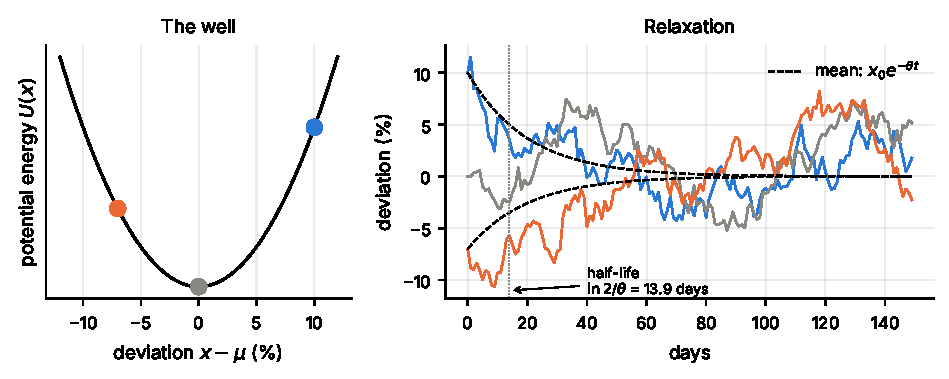
\includegraphics[width=0.95\textwidth]{fig3_pozo.pdf}
\caption{Left: the harmonic well $U(x)=\tfrac12k(x-\mu)^2$ with three starting points. Right: three
simulated paths with $\theta=0.05$/day and $\sigma=1\%$; dashed lines are the mean relaxation
$x_0e^{-\theta t}$.}
\label{fig:well}
\end{figure}

\subsection{Equilibrium is Boltzmann}

After a long time the particle forgets where it started. The Fokker--Planck equation for \cref{eq:ou},
\begin{equation}
\frac{\partial p}{\partial t}=\frac{\partial}{\partial x}\left[\theta(x-\mu)\,p\right]
+\frac{\sigma^2}{2}\frac{\partial^2p}{\partial x^2},
\end{equation}
has a drift term (the spring pulling in) and a diffusion term (noise spreading out). Setting the
probability current to zero gives
\begin{equation}
p_{\text{eq}}(x)\propto\exp\left[-\frac{\theta(x-\mu)^2}{\sigma^2}\right]
=\exp\left[-\frac{U(x)}{k_BT}\right],
\end{equation}
using $\theta=k/\gamma$ and $\sigma^2=2k_BT/\gamma$. It's the Boltzmann distribution in a harmonic well, a
Gaussian of width $\sigma/\sqrt{2\theta}$. With the numbers above that's $3.16\%$; a 3000-day simulation
gives $3.10\%$ (\cref{fig:boltzmann}).

\begin{figure}[ht]
\centering
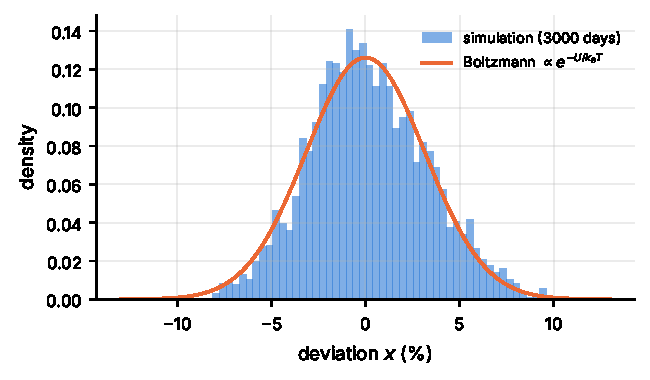
\includegraphics[width=0.62\textwidth]{fig3_boltzmann.pdf}
\caption{Histogram of a 3000-day simulated path and the predicted Boltzmann distribution.}
\label{fig:boltzmann}
\end{figure}

\subsection{Measuring the spring from data}

Sampling once a day, the exact solution of \cref{eq:ou} is
\begin{equation}
x_{t+1}-\mu=b\,(x_t-\mu)+\varepsilon_t,\qquad b=e^{-\theta}.
\end{equation}
Tomorrow's deviation is a fraction $b$ of today's, plus noise. So a linear fit of $x_{t+1}$ against $x_t$
gives $b$, and $\theta=-\ln b$. Small $b$ means a stiff spring, $b$ close to 1 a weak one, and $b=1$ no
spring at all (a random walk). On the 3000-day simulation (true $b=0.951$) the fit gives $b=0.949$,
$\theta=0.052$ and a half-life of $13.2$ days against the true $13.9$.

\subsection{Real data: is there a spring between the Nasdaq and the S\&P~500?}

Both indices track the US stock market, one with all large companies and one mostly with tech, so they
move together. Fitting $\ln(\text{Nasdaq})=1.34\,\ln(\text{S\&P})+c$ says that when the S\&P~500 goes up
$1\%$, the Nasdaq tends to go up $1.34\%$: tech amplifies market moves. What's left over is the spread
(\cref{fig:spread}).

\begin{figure}[ht]
\centering
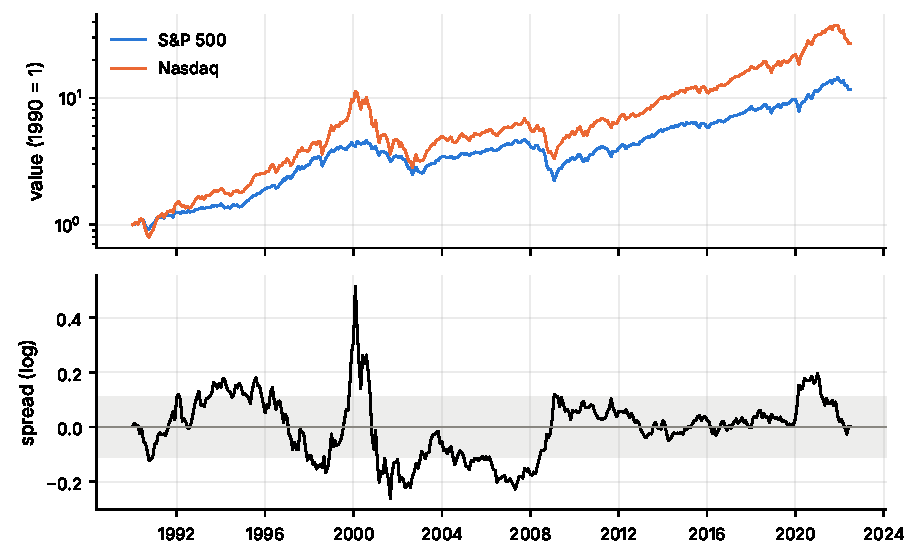
\includegraphics[width=0.95\textwidth]{fig3_spread.pdf}
\caption{Top: S\&P~500 and Nasdaq, 1990--2022 (relative to 1990, log scale). Bottom: the spread between
them; the grey band is one standard deviation.}
\label{fig:spread}
\end{figure}

With the regression above:
\begin{itemize}
\item the S\&P~500 alone has $b=0.997$ per month, a half-life of 216 months (18 years). For all practical
purposes, no spring, as expected for a price (\cref{sec:walk});
\item the spread has $b=0.956$, a half-life of 15 months. It looks like a spring.
\end{itemize}

This is where I had to be careful. The factor $1.34$ was chosen using the same data, precisely as the
combination that fits best, and that alone tends to produce a spread that seems to come back to zero even
when there is no spring. To check, I built 1000 pairs of \emph{independent} random walks, using the same
monthly steps as the two indices but shuffled, and ran exactly the same procedure on them. In $12\%$ of the
cases the fake pair gives a $b$ as small as the real one or smaller. So I can't claim the spring is real.

Looking at the figure it's clear why: the spread is dominated by a single episode, the dot-com bubble in
2000, when the Nasdaq went up about fivefold in a few years and then lost almost $80\%$. With a 15-month
half-life, thirty years of data only contain about twenty independent oscillations, and one of them weighs
too much. And a bubble isn't a spring phenomenon anyway. It's collective behaviour, which is the topic of
the last section.

This matters in practice too. \emph{Pairs trading} is a strategy that buys the relatively cheap asset and
sells the expensive one when the spread is stretched, betting on the spring. It only works if the spring
is real and stable, and checking that requires comparing with what chance alone would give.

% =====================================================================
\section{Herding, bubbles and crashes: the Ising model}
\label{sec:ising}
% =====================================================================

\subsection{Market version first}

A \emph{bubble} is a price rise far beyond what the company's profits can justify: people buy because the
price goes up, and the price goes up because people buy. A \emph{crash} is the opposite, a sudden
collective fall, often without a single piece of news that explains it. Both have one thing in common:
many investors doing the same thing at the same time. Nobody decides to buy into a bubble in isolation;
people look at what others are doing and copy them, the same way we pick the restaurant that's already
full \cite{kirman1993}.

\subsection{Physics: spins that align}

The Ising model describes a magnet as a lattice of spins $s_i=\pm1$, each one preferring to point like its
neighbours (coupling $J>0$) and like the external field $h$:
\begin{equation}
E=-J\sum_{\langle ij\rangle}s_is_j-h\sum_is_i .
\end{equation}
At low temperature energy wins and the spins align: spontaneous magnetization. At high temperature entropy
wins (there are vastly more disordered configurations than ordered ones) and the magnetization vanishes.
In between there's a critical temperature $T_c$ \cite{uam_me3}.

\subsection{The translation}

Each spin is an investor: $s_i=+1$ buys, $s_i=-1$ sells. The magnetization
\begin{equation}
m=\frac1N\sum_is_i
\end{equation}
is the fraction of buyers minus the fraction of sellers, i.e.\ the \emph{excess demand}. With $m=0.5$, 75\%
buy and 25\% sell. Since excess demand is what moves the price, in the simulations I use the simplest
possible link: each day the log-price changes in proportion to $m$, $\ln P_{t+1}=\ln P_t+\lambda m_t$.

\begin{table}[ht]
\centering\small
\caption{Dictionary for this section.}
\begin{tabular}{@{}ll@{}}
\toprule
Physics & Market \\
\midrule
spin $s_i=\pm1$ & investor buying ($+1$) or selling ($-1$)\\
magnetization $m$ & excess demand\\
coupling $J$ & tendency to copy others\\
external field $h$ & news affecting everyone (good if $h>0$)\\
temperature $T$ & diversity of opinions, independent decisions\\
ordered phase ($T<T_c$) & consensus: bubble or panic\\
susceptibility $\chi$ & sensitivity of the market to news\\
hysteresis & the market doesn't come back the same way it went\\
\bottomrule
\end{tabular}
\end{table}

The temperature needs a comment. In the magnet it's thermal agitation. Here it stands for everything that
makes investors decide on their own: private information, different needs (someone sells because they need
the cash, not because they expect a drop), different opinions. A ``hot'' market in this sense is a
diverse one, and that makes it stable. It's not the same temperature as in \cref{sec:temp}, which measured
how much prices move. In fact they're almost opposite: little diversity of opinion leads to very agitated
prices.

\Cref{fig:spins} shows the model on a square lattice where each investor only copies four neighbours (say,
the people they talk to). Below $T_c$ almost everyone buys; near $T_c$ there are clusters of all sizes;
above it everyone does their own thing.

\begin{figure}[ht]
\centering
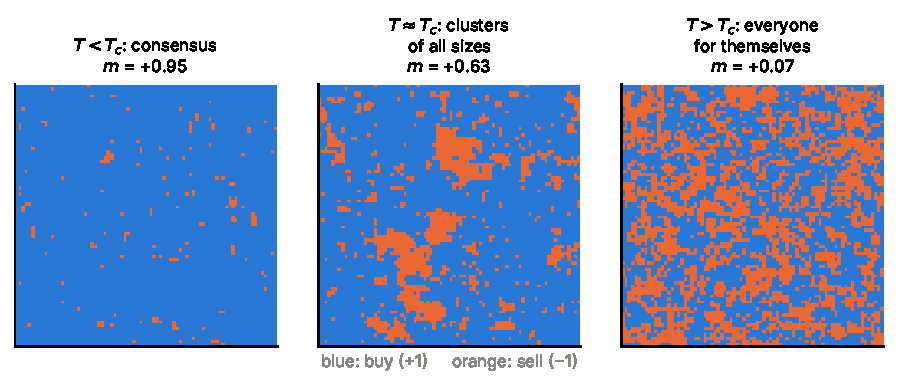
\includegraphics[width=0.95\textwidth]{fig4_espines.pdf}
\caption{Ising model on an $80\times80$ lattice, starting with everyone buying, at three temperatures (on
this lattice $T_c=2.27\,J$).}
\label{fig:spins}
\end{figure}

\subsection{Mean field: everyone looks at the average}

In a real market nobody only sees four neighbours: everyone sees the price, which summarizes what everyone
is doing. So I use the mean-field version, where each investor feels the average opinion of the others.
The field on investor $i$ is $Jm+h$: peer pressure plus news. At temperature $T$ the probability of buying
is the Boltzmann one for a spin in that field, and the mean is $\langle s_i\rangle=\tanh[(Jm+h)/T]$. But the
mean of each $s_i$ is $m$ by definition, which gives the self-consistency equation
\begin{equation}
m=\tanh\left(\frac{Jm+h}{T}\right).
\label{eq:weiss}
\end{equation}
Everyone's opinion depends on everyone else's, and $m$ appears on both sides.

\Cref{fig:meanfield} (left) solves it graphically for $h=0$. The slope of $\tanh(Jm/T)$ at the origin is
$J/T$. For $T>J$ the curve is flatter than the diagonal and the only solution is $m=0$: buyers and sellers
balance out. For $T<J$ two more solutions $\pm m_0$ appear: \emph{consensus without any news}. So
$T_c=J$. At $T=0.9\,J$, for example, $m_0=0.53$, meaning 76\% of investors buy (or sell) simply because the
others do.

\begin{figure}[ht]
\centering
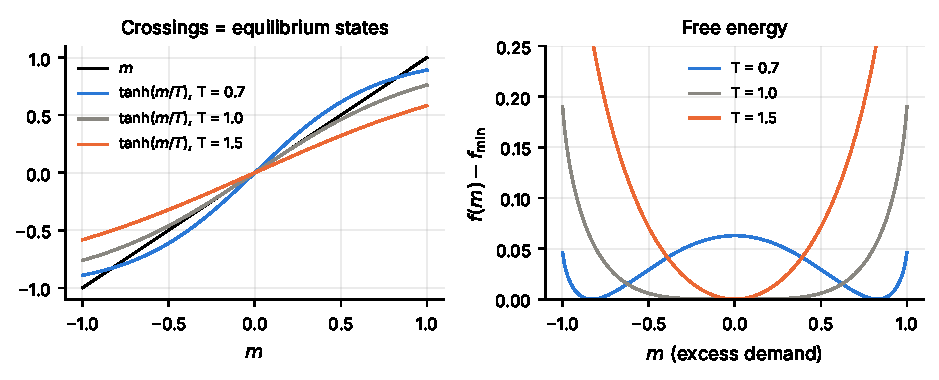
\includegraphics[width=0.95\textwidth]{fig4_campo_medio.pdf}
\caption{Left: graphical solution of $m=\tanh(m/T)$ with $J=1$; equilibria are the crossings with the
black diagonal. Right: free energy per investor at the same three temperatures.}
\label{fig:meanfield}
\end{figure}

\subsection{Energy against entropy}

The same story in terms of the free energy per investor (\cref{fig:meanfield}, right):
\begin{equation}
f(m)=-\frac{J}{2}m^2-hm-T\,s(m),\qquad
s(m)=-\frac{1+m}{2}\ln\frac{1+m}{2}-\frac{1-m}{2}\ln\frac{1-m}{2}.
\end{equation}
The first term rewards consensus. The entropy counts in how many ways a given excess demand can be
realized: there are enormously many ways to have half buyers and only one way for everyone to buy. At high
temperature entropy wins and the minimum is at $m=0$. Below $T_c$ copying wins and two valleys appear, an
optimistic one and a pessimistic one, separated by a barrier.

\subsection{Three simulated markets}

To see what this means for prices, I simulated a market of 150 investors who update their decision one at
a time with the Boltzmann rule above, plus a small random piece of news $h$ every day. \Cref{fig:markets}
shows excess demand and price at three temperatures.

\begin{figure}[ht]
\centering
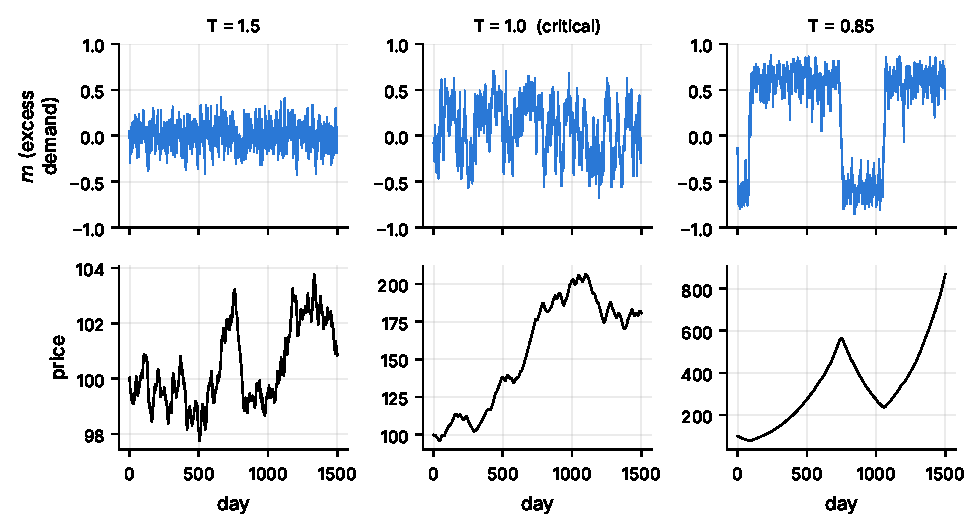
\includegraphics[width=0.95\textwidth]{fig4_mercados.pdf}
\caption{Simulated Ising market over 1500 days. Top: excess demand $m$. Bottom: price, which changes
every day in proportion to $m$. Left: lots of diversity ($T=1.5\,J$). Middle: at the critical point. Right:
herding dominates ($T=0.85\,J$).}
\label{fig:markets}
\end{figure}

At $T=1.5\,J$, excess demand fluctuates around zero and the price looks like a random walk, the market of
\cref{sec:walk}. At the critical point $T=J$, fluctuations of $m$ become large and slow, and the price moves
in long trends that build up and fade away without any important news; the one-day autocorrelation of $m$
goes from $0.69$ to $0.94$. At $T=0.85\,J$ the market gets stuck for hundreds of days in one of the two
valleys, so the price either climbs steadily (a bubble) or falls steadily. Every now and then a fluctuation
carries it over the barrier and the consensus flips: a crash. There are 3 such flips in 1500 days.

\subsection{Susceptibility: small news, big effects}

How much does excess demand change when news arrives? That's the susceptibility $\chi=\partial m/\partial h$.
Linearizing \cref{eq:weiss} around $m=0$ gives, above $T_c$,
\begin{equation}
\chi=\frac{1}{T-T_c},
\end{equation}
which diverges at the critical point (Curie--Weiss law). In the simulation I don't need to apply any news to
measure it: by fluctuation--dissipation, the response to a push is proportional to the spontaneous
fluctuations, $\chi=N\,\mathrm{Var}(m)/T$. \Cref{fig:response} (left) shows it follows the prediction:
$\chi=1.03$ at $T=2J$ (theory: 1) and $\chi=7.6$ at $T=1.1J$ (theory: 10, the gap comes from the finite
number of investors).

In market terms: in a diverse market a piece of news has an effect proportional to its importance. Near
the critical point, where everyone watches everyone else, the same news gets amplified out of proportion,
because each investor who reacts drags others along.

\begin{figure}[ht]
\centering
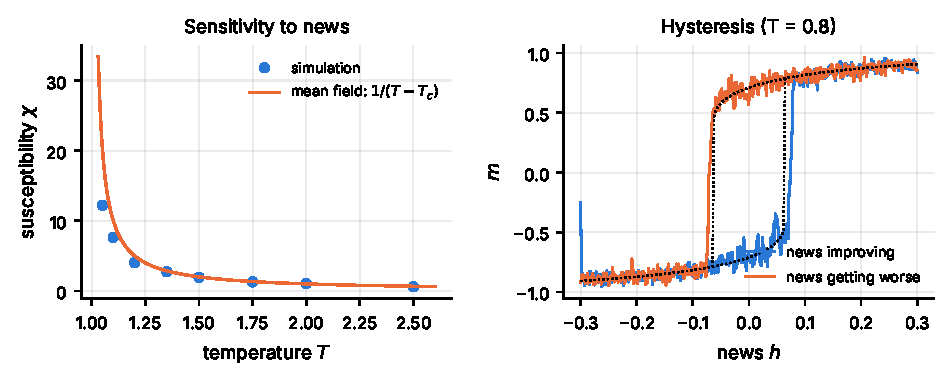
\includegraphics[width=0.95\textwidth]{fig4_respuesta.pdf}
\caption{Left: susceptibility from the simulation and the mean-field prediction. Right: excess demand when
the news slowly improves (blue) and then gets worse (orange), at $T=0.8\,J$. Dotted lines: the two branches
of the mean-field solution.}
\label{fig:response}
\end{figure}

\subsection{Hysteresis: a crash as a first-order transition}

The last experiment is my favourite. At $T=0.8\,J$ I start with bad news ($h=-0.3$), which leaves the
market in the pessimistic valley, then improve the news very slowly up to $h=+0.3$, and then make it worse
again just as slowly (\cref{fig:response}, right).

When the news turns good ($h>0$), the market \emph{stays pessimistic}. The pessimistic valley is no longer
the deepest one, but the market is inside it and nothing pushes it out. Only when the news is clearly good,
$h\approx0.07$, does that valley disappear and the market jumps to optimism all at once. Mean-field theory
says the valley disappears at $h=0.062$; the simulation jumps at $h=0.074$. On the way back the same thing
happens in reverse: optimism survives bad news until $h\approx-0.06$, and then it collapses.

This is supercooled water, which can stay liquid below $0\,^\circ$C until it suddenly freezes all at once.
For markets it says something I find genuinely useful: \emph{a crash doesn't need terrible news}. It only
needs a series of small bad news, each one harmless, that brings the system to the edge of the valley. The
last drop is no bigger than the previous ones; it just arrives when the valley is already gone. And the
other way round, a market coming from widespread pessimism can take a long time to react to good news.

\subsection{Limitations}

This is a deliberately simple Ising: all investors are identical, everyone sees everyone, and the price
responds linearly to excess demand. More realistic versions mix investors that copy others with
investors that buy when the price looks cheap and sell when it looks expensive, and those reproduce both
the fat tails and the volatility clustering of \cref{sec:temp} \cite{bornholdt2001}. People have also tried
to use the critical point to anticipate crashes \cite{sornette2003}, with mixed results. What the simple
model does show clearly is the mechanism: copying plus shrinking diversity leads to large, slow
fluctuations and occasional abrupt jumps.

% =====================================================================
\section{Summary and next steps}
% =====================================================================

The four ideas fit together. The random walk describes the day-to-day behaviour well: no memory, and risk
growing like the square root of time. It fails on extreme days, and temperature explains why: the market
alternates between cold and hot periods, and mixing temperatures produces fat tails. The spring describes
quantities that do come back, but showing that a spring really exists takes a comparison with chance. And
the Ising model shows how copying between investors can produce bubbles, crashes and an exaggerated
response to news.

\begin{table}[ht]
\centering\small
\caption{What the data say.}
\label{tab:summary}
\begin{tabular}{@{}p{3.0cm}p{5.2cm}p{5.4cm}@{}}
\toprule
Idea & Prediction & Result\\
\midrule
Random walk & no memory; variance $\propto t$; Gaussian & yes; yes (slope 1.10); no, fat tails\\
Temperature & clustering; tails from mixing; predictable temperature & yes ($C_{|r|}(1)=0.15$); partly; yes, out of sample\\
Spring & deviations decay with a fixed half-life & yes in simulation; inconclusive for Nasdaq--S\&P ($p=0.12$)\\
Ising & consensus, diverging susceptibility, hysteresis & reproduced in simulation\\
\bottomrule
\end{tabular}
\end{table}

Things I'd like to try next: running the same analysis on many stocks and on minute-by-minute data, which
would multiply the number of observations by hundreds; looking for pairs of assets whose spring actually
passes the random-walk test; and fitting an Ising model with several types of investors to real data, to
see whether its distance to the critical point says anything about upcoming crises.

% =====================================================================
\appendix
\section{Running the code}
% =====================================================================

The repository has five Python files. \texttt{comun.py} loads the data and sets the plotting style; the
other four match the four sections and run independently:
\begin{verbatim}
pip install -r requirements.txt
python 01_paseo_aleatorio.py
python 02_temperatura.py
python 03_muelle.py
python 04_ising.py
\end{verbatim}
Each script saves its figures and prints every number quoted in this document. By default the figure
labels are in Spanish and go to \texttt{figuras/}; running with \texttt{IDIOMA=en} (for example
\texttt{IDIOMA=en python 01\_paseo\_aleatorio.py}) produces the English figures used here, in
\texttt{figures/}. The code comments are in Spanish. To analyse a different stock, change the loading
function in \texttt{comun.py}.

\bibliographystyle{unsrt}
\bibliography{references}

\end{document}
